\chapter{Social network boosted search ranking}

Charles Explorer is an academic search engine, which allows the user to search for publications, classes, people and study programmes in the academic domain.

The following sections, we look more into the search engine part of the application, explore the possible issues with the search results ranking, 
and experiment with utilizing the social network data for the search results ranking improvement.

\section{Full-text search}

Full-text search is nowadays an essential part of any information retrieval system. 
Many search engines - including Apache Solr in Charles Explorer - implement the full text search by utilizing the TF-IDF algorithm.
This is a simple and efficient way to rank the search results based on the relevance of the documents to the search query.

The TF-IDF algorithm is based on the term frequency and inverse document frequency of the terms in the documents - a \textit{document} is in general unstructured free text content.
Some entities in our academic search engine map well to this notion of a \textit{document} - e.g. a \texttt{publication} or \texttt{class} both have inherent textual content (titles, abstracts or syllabi).
Unfortunately, this does not hold for all the entities in the system.

As an example, a \texttt{person} entity usually does not have any explicit textual content associated with it. 
When searching for a person interested in a particular topic, the search engine has to rely on the textual content of the publications, classes, 
or other entities associated with the person, i.e. traverse - at least implicitly - the knowledge graph (or the social network of the person).

A simple solution to this problem would be to represent every person as a document, concatenating all the textual content of the entities associated with the person.
This can be further refined by assigning different weights - e.g. to the different types of entities (a \texttt{class} might be more important than a \texttt{publication}), 
or different concatenated parts of the documents (e.g. the publication title and class name are more important than the abstracts and syllabi).

Regarding adding new entities related to a given person, the concatenation also serves us well - we can simply append the new entity's content to the person's document and reindex it.

However, this approach also has several drawbacks. First of all, assuming we're building a general academic search engine allowing for search in publications, classes and people, we would be indexing the same content multiple times.
This is not only inefficient in terms of storage, but also prone to update errors - there is multiple copies of the same content, which have to be updated separately.
The second issue arises from the concatenation - if any of the person's associated entities changes, the whole document has to be reindexed.
However, this might be less of a problem than the first issue, as it's not too common for academic records to get updated or removed - at least in comparison to the number of new records being added.

\subsection{Result ranking in the naive case} \label{search-ranking-issues}

Result ranking in information retrieval refers to the ordering of the search results when presented to the end user. This is often based on the relevance of the documents to the current search query.
The relevance-based ranking is often enough for the basic use case - the user is presented with the most relevant documents first, and can further explore the less relevant ones if needed.

While it might seem a bit superficial, the ranking is in fact still part of the information retrieval process. 
As multiple studies show \footnote{https://link.springer.com/article/10.1007/s11151-014-9435-y}\footnote{https://link.springer.com/article/10.1007/s10791-010-9150-8}, 
the ranking of the search results positively correlates with the click-through rate of the results 
- likely because of the typical top-left to bottom-right reading pattern of the users.
This can be further affected by other, more technical factors - such as the need for an additional user action like scroll or pagination to see the results further down the list.

%% https://link.springer.com/article/10.1007/s10791-010-9150-8 - Re-ranking search results using an additional retrieved list

Considering a simple tf-idf based search engine, the ranking of the search results is based on the relevance of the documents to the search query.
This is directly related to the term frequency of the query in the document - for a fixed query and a given document collection, we can forget about the inverse document frequency, as it's constant over all the documents.
Ranking the documents solely based on the term frequency might however lead to unfavourable results - especially in the case of a proxy-representation of a given entity.


\begin{figure}[ht!]
    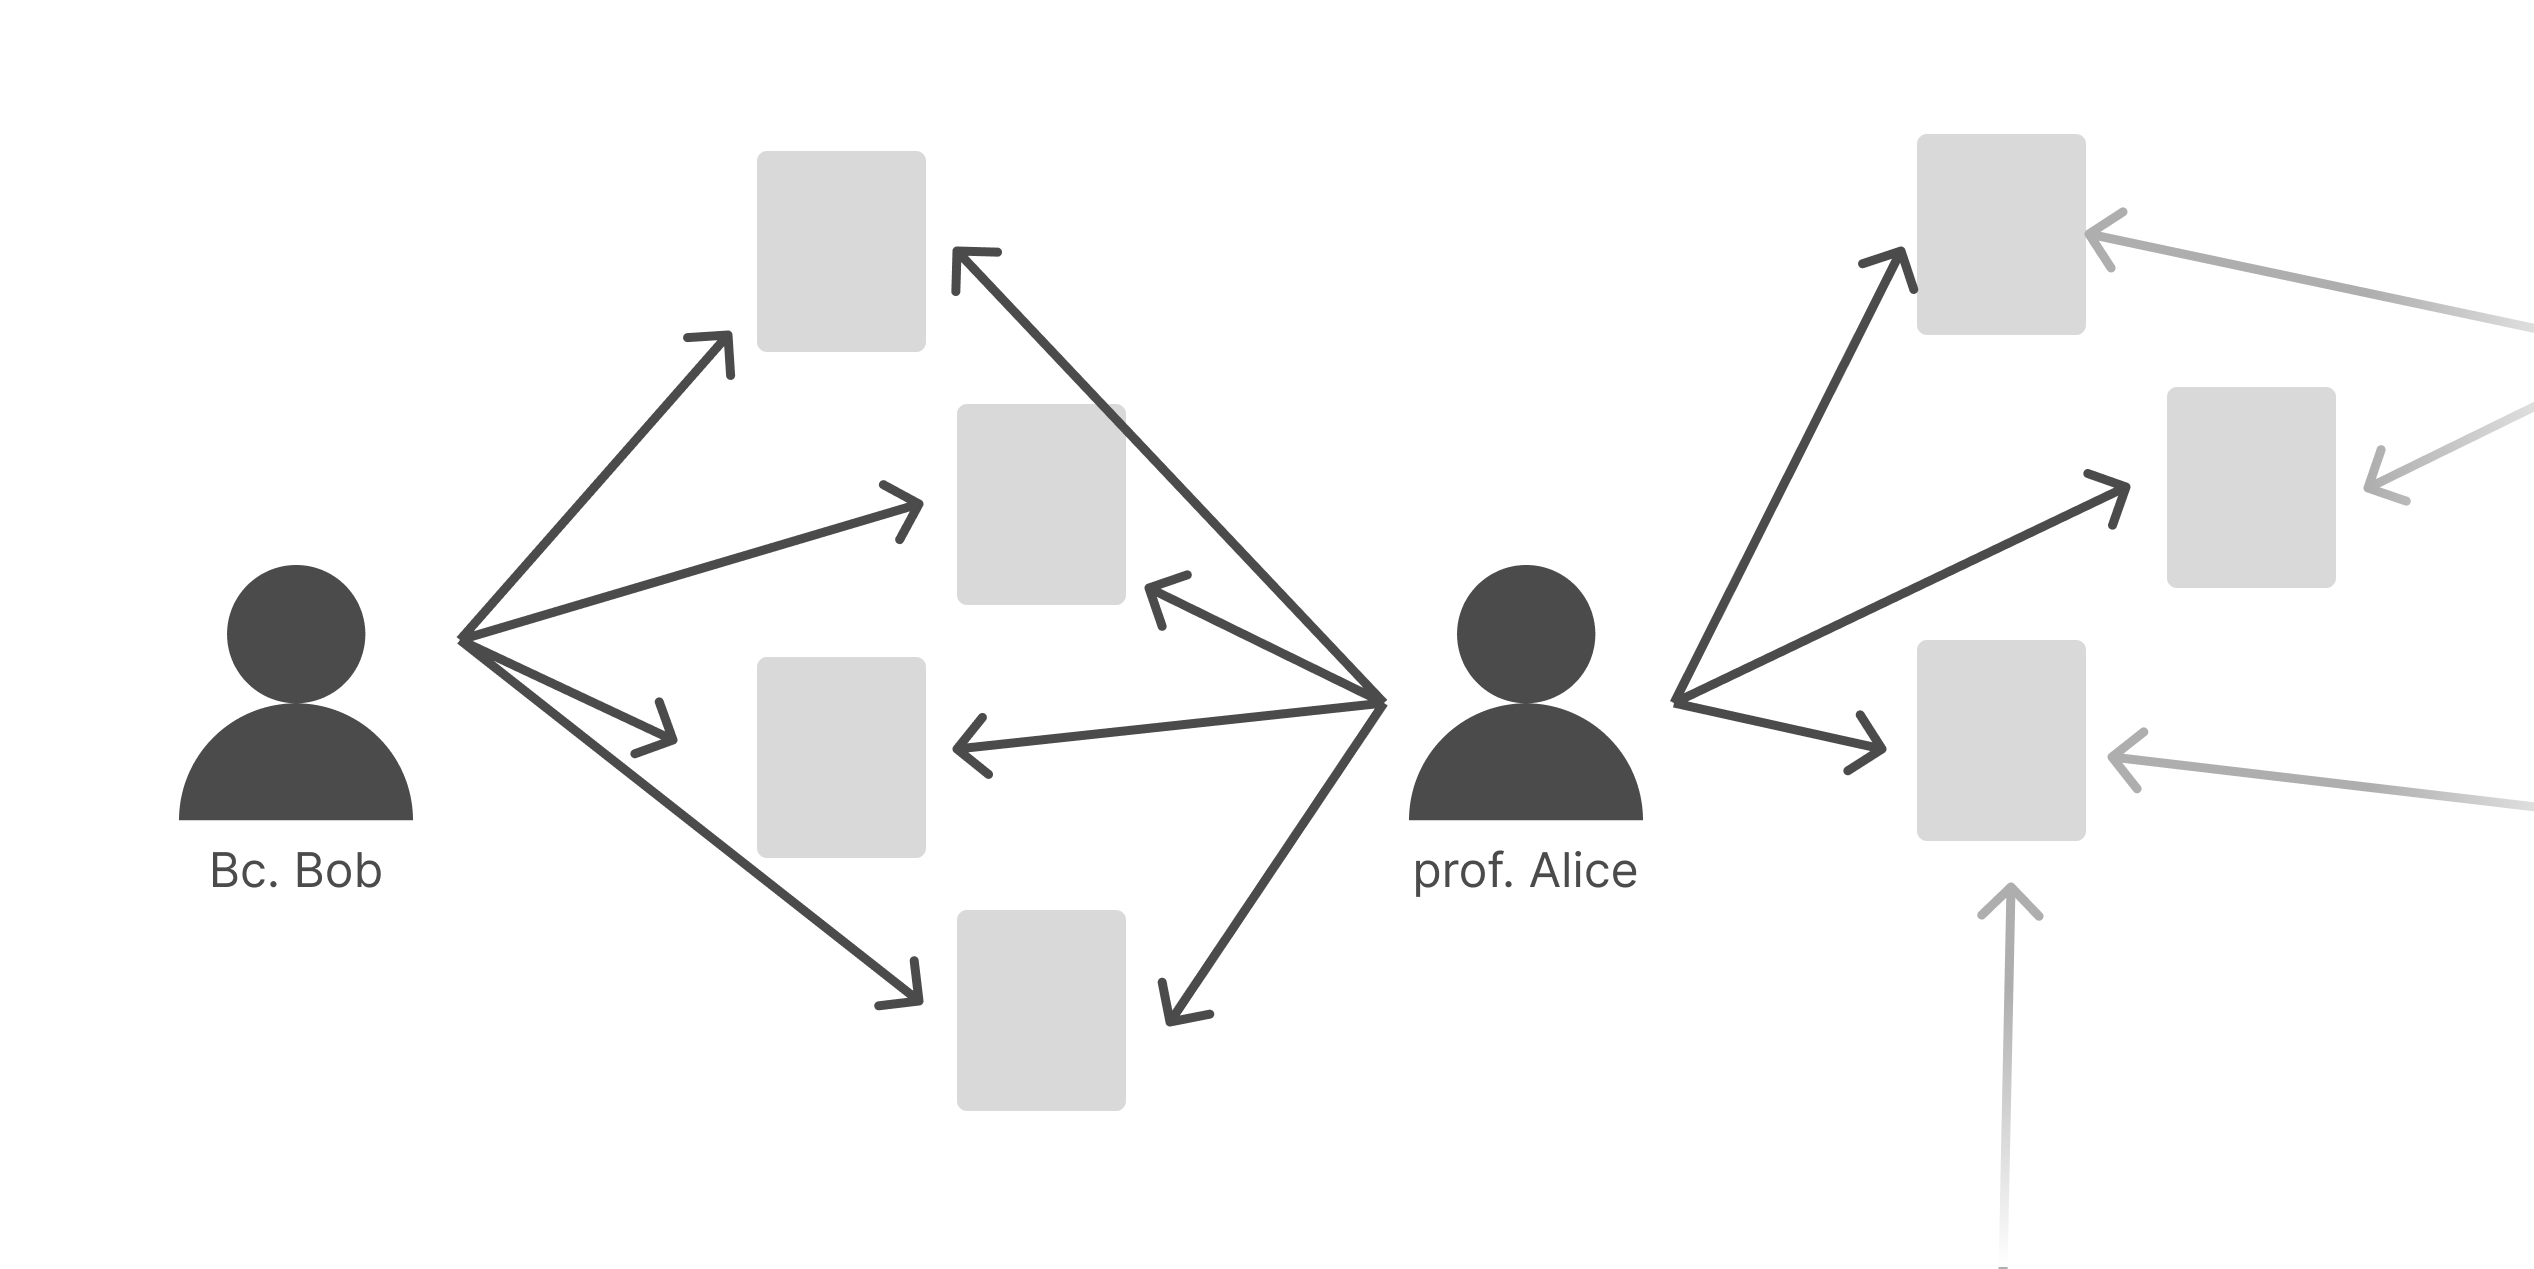
\includegraphics[width=0.8\textwidth]{../img/bob-alice-soc-netw.png}
    \centering
    \caption{Simple representation of the social network of Alice and Bob.}
\end{figure}

Let us explore the issues on an example where we represent people as documents, concatenating the textual content of the entities associated with them.
Consider two academic researchers in our system - \textit{prof. Alice} and \textit{Bc. Bob}. 
Bob is a student of Alice, and has published several papers on \textit{Information retrieval} with her. Aside from those, Bob has not published any other papers.
On the other hand, Alice has published a lot of papers on various topics - related to IR, but also to other similar fields. 
See a simple representation of their social network above.

Note that aside from the common publications, Bob has no other entities associated with him, while Alice has other publications with other co-authors.

\begin{figure}[ht!]
    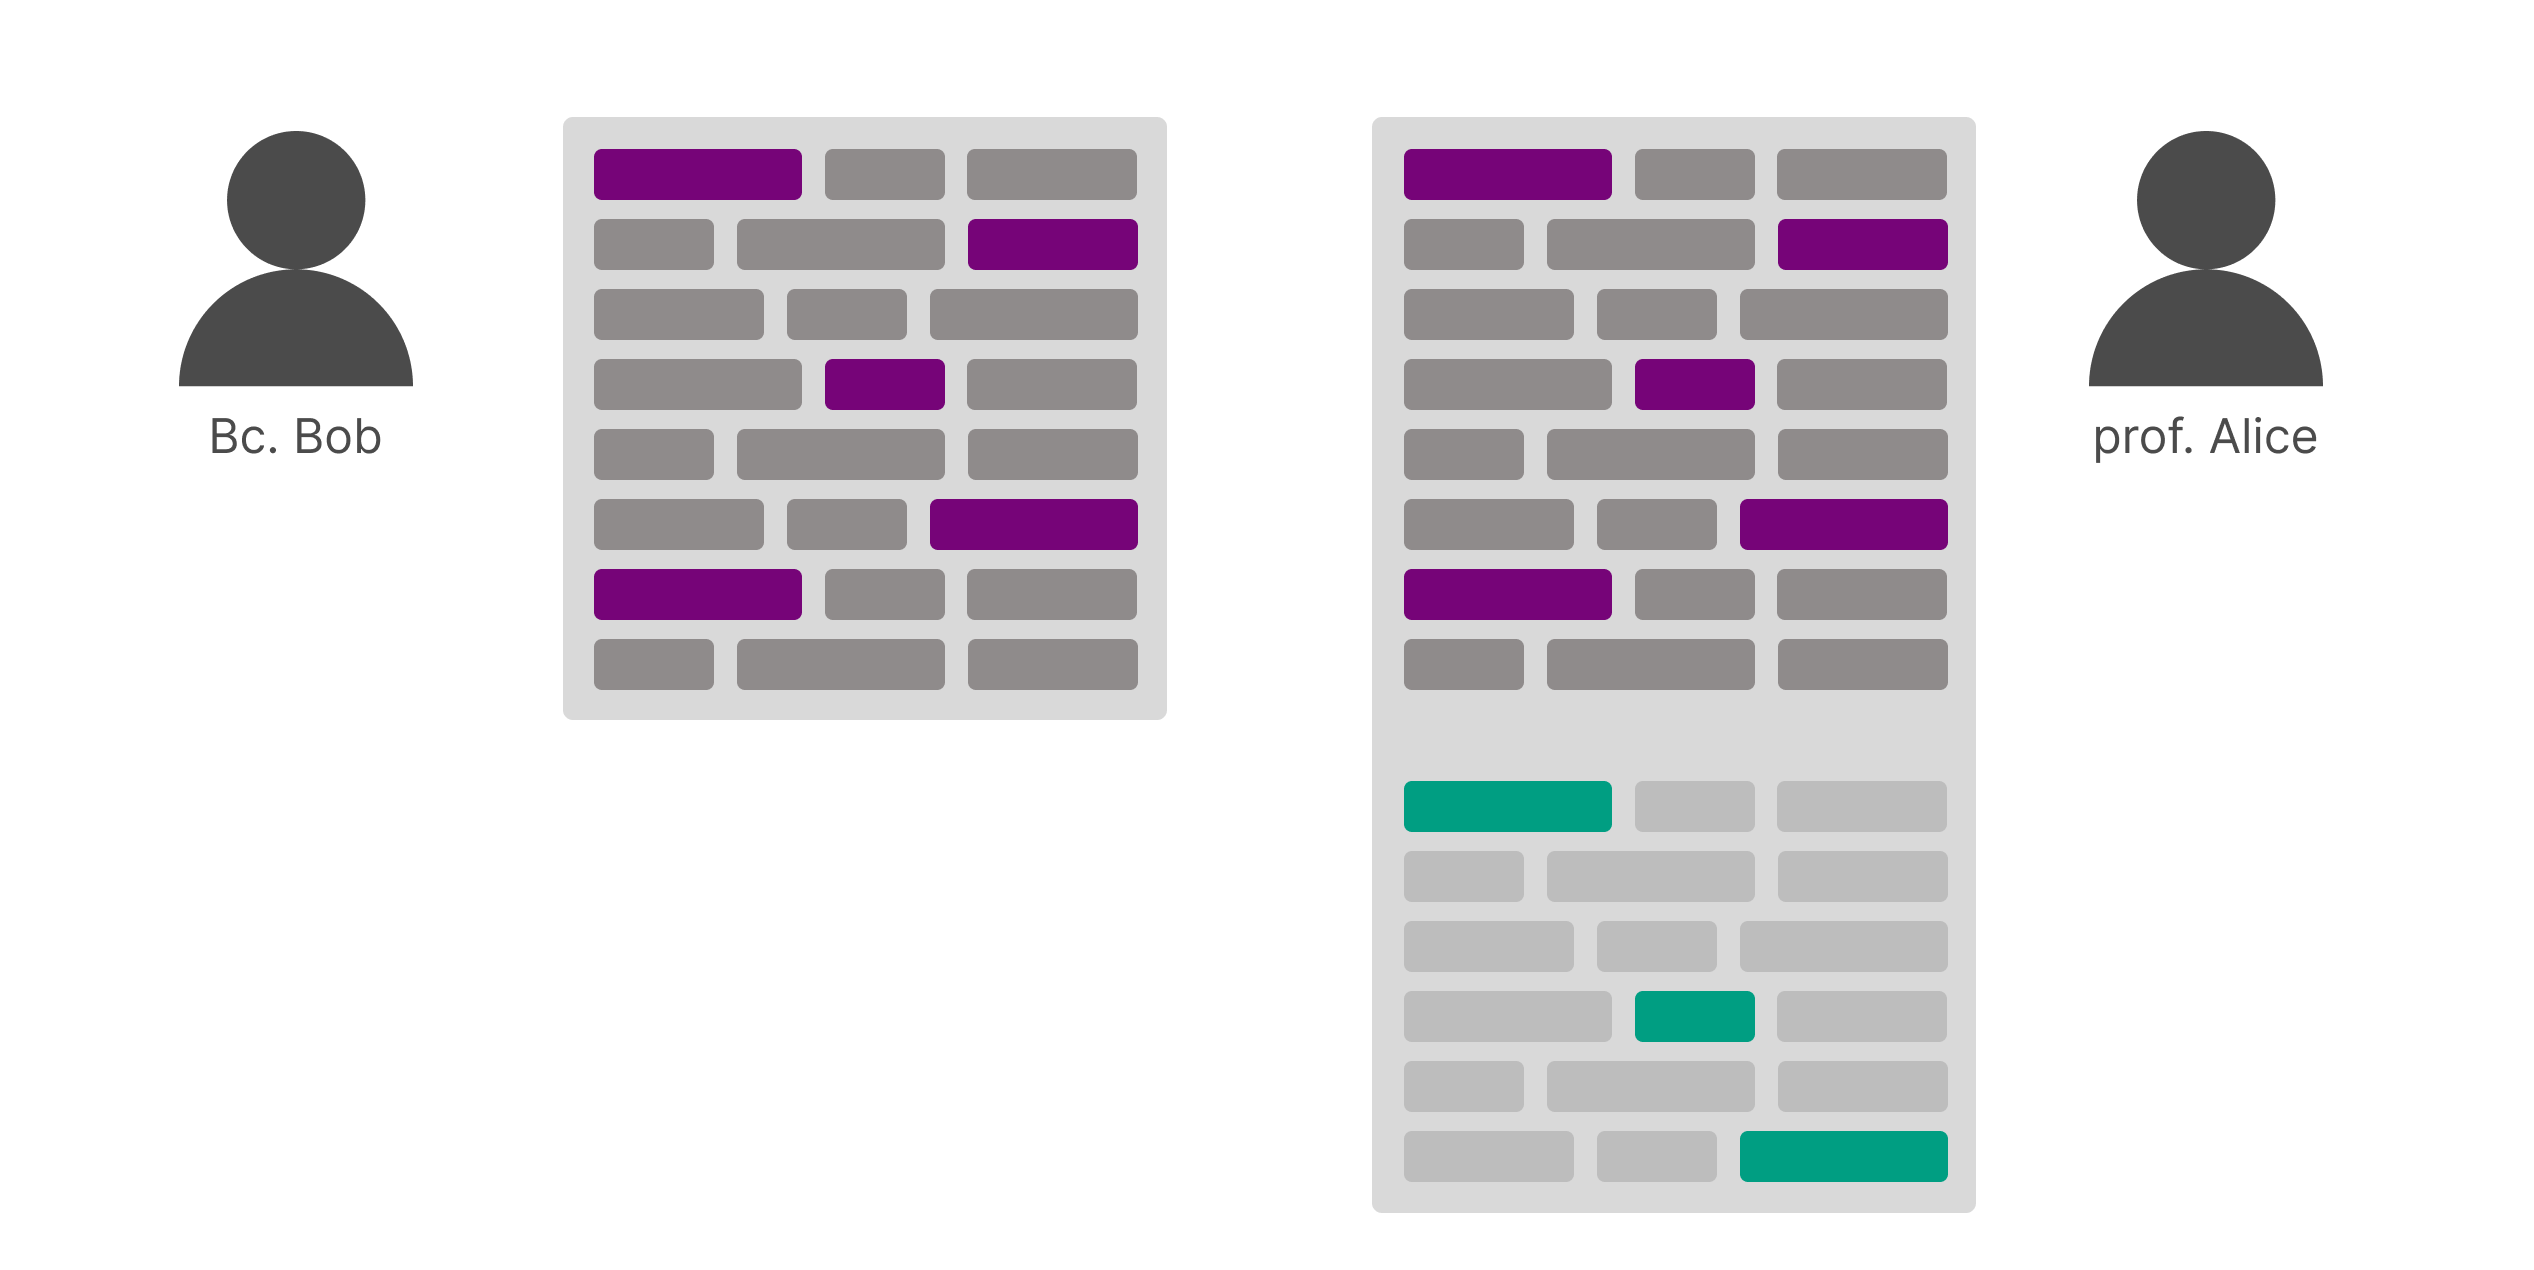
\includegraphics[width=0.8\textwidth]{../img/bob-alice-representations.png}
    \centering
    \caption{Concatenating representations of Alice and Bob as documents.}
\end{figure}

We see that the document of Bob is shorter than the one of Alice, because he has less associated entities. We can also notice that the Alice's document fully contains the Bob's document.
    
The colored terms represent the current search query - if Alice only published papers on the topic of the query with Bob, the term frequency of the 
query in Bob's document would be strictly higher, because of the shorter length.
In case Alice also publishes on the topic with other co-authors, it gets harder to reason about which of the term frequencies is higher.

The relation between the tf-idf scores of the documents of Alice and Bob can be expressed as follows:
\begin{subequations}
\begin{align}
\text{tf}(q, d_{\text{Bob}}) \times \text{idf}(q, D) &\stackrel{?}{>} \text{tf}(q, d_{\text{Alice}}) \times \text{idf}(q, D) \\
\text{tf}(q, d_{\text{Bob}}) &\stackrel{?}{>} \text{tf}(q, d_{\text{Alice}})
\end{align}
\end{subequations}

Normalized term frequency $\text{tf}_{q,d}$ of a term $q$ in a document $d$ is defined as the number of times the term $q$ appears in the document $d$ (denoted by $f_{q,d}$),
divided by the total number of terms in the document $d$ (the document's length).

\begin{subequations}
\begin{align}
\frac{f_{q, d_{\text{Bob}}}}{\text{len}(d_{\text{Bob}})} &\stackrel{?}{>} \frac{f_{q, d_{\text{Alice}}}}{\text{len}(d_{\text{Alice}})} \Biggm/ \;^{-1} \\
\frac{\text{len}(d_{\text{Bob}})}{f_{q, d_{\text{Bob}}}} &\stackrel{?}{<} \frac{\text{len}(d_{\text{Alice}})}{f_{q, d_{\text{Alice}}}} \Biggm/ \textit{assuming that } \mathit{f_{q, d_{\text{Bob}}} = f_{q, d_{\text{Alice}}}} \label{eq:51assumption}\\
\text{len}(d_{\text{Bob}}) \;&<\;\text{len}(d_{\text{Alice}})
\end{align}
\end{subequations}

Since we have assumed that Alice's document is a superset of Bob's document, the result inequality holds - and therefore the tf-idf score of Bob's document is higher than the one of Alice's document.

Note that the assumption in the equation \ref{eq:51assumption} is only true for the cases when Alice does not publish any other papers on the topic of the query with other co-authors.

% Because of this, the document representation of Bob will be short, compared to the one of Alice.
% Assuming the search query is \textit{Information Retrieval} - and there are no other publications or classes related to this topic in the system - 
% the search engine will consider Bob as the more relevant person for this topic. This is becuase the term frequency of the query in Bob's document is higher than in Alice's document - solely because of the length.

In either way, this approach most likely will not provide the desired outcome - while Bob has published papers only on the given topic - and therefore has higher ``tf-idf relevance'' to the query,
it is likely that Alice is the more relevant person for the searching user, since she is more experienced in the topic.

\section{Re-ranking}

In the following sections, we go over different existing re-ranking strategies utilized in other systems and explore the possibilities of using the social network data for the re-ranking in Charles Explorer.

\subsection{Existing re-ranking strategies}

In the current (2024) commercial search engines, there are often multiple re-ranking strategies available to the users.
Unfortunately, only a small portion of the engines actually discloses the details of the re-ranking algorithms used - perhaps to protect the intellectual property and the competitive advantage.

The common grounds for all those systems is the two-stage search pipeline - in the first stage, a traditional search engine is used to retrieve the initial set of results.
Then, these results are re-ranked using a different algorithm. 

While it might seem redundant, this approach allows the second algorithm to focus only the more relevant results, and be perhaps more computationally expensive.
Unfortunately, this also means that the re-ranking algorithm is not able to affect the initial search results - it can only change the order of the results.
It also brings in the issue of pagination - if the user has to go through multiple pages of the search results, the re-ranking might not be as effective,
as it only affects the current page of the results.

The re-ranking algorithms can be based on various factors - the user's previous interactions with the system, total popularity (click-through rate) of the items,
diversity of the results %link to the MMR papers https://www.google.com/search?client=firefox-b-lm&q=Maximal+Marginal+Relevance 
or NLP analysis of the documents. Especially the last one seems to be gaining traction in the recent years, as the applications of LLM models are becoming more widespread.

\subsection{Graph data-based reranking}

As we discussed in \ref{search-ranking-issues}
, the traditional tf-idf based search engine might give unsatisfactory results in the case 
of a proxy-representation of a given entity.
We might try to address this issue by utilizing the social network data for the re-ranking of the search results.

As mentioned in the previous subsection, many commercial search engines use a two-step search pipeline - the first step retrieves the initial set of results,
and the second step re-ranks them using a different algorithm. This sounds like a good fit for our problem - we can use the traditional tf-idf based search engine 
to retrieve the initial set of results, and then re-rank them using the social network data. 

Only using the graph data for the search has several drawback described in the next section (\ref{graph-based-search}).

When it comes to reranking the existing search results, we can utilize the social network data in several ways.

\begin{itemize}
    \item \textbf{Global node statistics}: As illustrated on the example of Alice and Bob above, 
    we can use the global statistics for the nodes in the social network to re-rank the search results. 
    These include - but are not limited to - the node degree (number of connections), centrality measures, or the number of common neighbours.

    Such statistics can be precomputed for every node in the social network before the search and stay constant over all the search queries.

    \item \textbf{Query relevant node statistics}: Unlike the global node statistics, query-relevant node statisics are computed only for the nodes in the search results.
    
    These can perhaps define the node's relevance better (e.g. the number of query-relevant publications connected to a given person), but are often more computationally expensive to compute.
    Given the variability of the queries, it is also harder (or impossible) to precompute these statistics.
\end{itemize}

%% todo structure
\subsection{Graph data-based search} \label{graph-based-search}

It would also be possible to use the social network data to entirely replace the concatenated person representations in the search engine - we could 
only search through the ``first-order entities'' (i.e. classes and publications) and then query the social network graph for the people associated 
with the results of the search. 

This approach has several drawbacks - aside from the questionable performance and scalability / developer effort, it also might not be as effective as the concatenated representation.

With the concatenated approach, we have to retrieve only \textasciitilde{} 30 results (people) for every page of the search results. 
Those are also already ranked by the relevance to the query - even though this might not be perfect, the tf-idf based ranking is still a good approximation.

With the proposed graph-based approach, we would have to retrieve many more publications and classes on each search - note that we are no longer 
looking for the most-relevant class or publication, but for the most-relevant person - which is rather an aggregation of the relevance of the associated entities.
This might lead to a lot of unnecessary data retrieval and processing and become the bottleneck for the possible applications built on such data.


\section{Benchmarks}

To determine the performance of our proposed re-ranking solution, we establish a set of benchmarks to compare the results of the traditional tf-idf based search engine with the social network enhanced search engine.

The common denominator for many of the ranking measuers is the \textit{user interaction} - the user is presented with the search results and picks the most relevant one or scores the 
results based on the relevance to the query.

Unfortunately, this is not applicable to our case - while we are tracking the user interactions in the Charles Explorer web appplication, the amount of collected data is far too low to be statistically significant.

\subsection{Acquiring gold standard data}

To establish a gold standard for the search results relevance (and by proxy the ranking), we do not have to rely on human interactions.

Elsevier Scopus\footnote{https://www.elsevier.com/products/scopus} is a large academic database, which provides a search engine for the academic publications.
Aside from the web application, it also provides a REST API for consuming the data programmatically.

Clarivate's Web of Science\footnote{https://www.webofscience.com/} is another large academic database, providing a similar service as Scopus above.

Since both of the applications are search engines for the academic publications, we can use their ranking and search results as the gold standard for our benchmarks.

\section{Implementation details, performance}

A section about the implementation details for the social network enhanced search within Charles Explorer. Can contain parts about the actual real-time performance (and discussion whether the added reranking value is worth the potential performance degradation).

\dots

